\section{Methoden und Arbeitstechniken}
\subsection{Pair Programming}
Pair Programming (im deutschen Paarprogrammierung) ist eine Methode in der Softwareentwicklung, in welcher die Entwicklung einer Aufgabe von 2 Personen vollzogen wird. Bei der Entwicklung existieren in diesen Paar 2 Rollen:
\begin{enumerate}
	\item Jemand der programmiert
	\item Ein Beobachter, welcher das programmierte überprüft und im Fall eines Problems/Fehlers direkt Feedback gibt
\end{enumerate}
Die Besetzung der Rollen sollte möglichst häufig wechseln. Ein Vorteil dieser Methode ist die Reduzierung von Fehlern, da durchgängig ein Review durch einen anderen Teilnehmer statt findet und hilft somit bei einer schnelleren Fehlerbehebung. Aber auch der Lerneffekt (besonders bei einen Studentenprojekt) ist immens, da neue Techniken direkt an andere Personen weiter getragen wird. Ein weitere wichtiger Punkt neben dem Tausch der Besetzungen bei den Rollen, ist das Durchtauschen der Paare, damit jeder von anderen Teilnehmern des Projektes lernen kann.

\subsection{Planning Poker}
Planning Poker ist eine gamifizierte Methode, um Projektaufgaben ( in unseren Fall User Stories) zu schätzen. Ein wichtiger Punkt beim Planning Poker ist, dass alle Teilnehmer zuerst ihre Schätzung vornehmen bevor man die anderer Teilnehmer sieht. Dadurch schließt man eine Beeinflussung durch andere Schätzungen aus und erhält somit einen besseren Überblick. Ein weiterer wichtiger Punkt ist, dass Schätzungen in so genannten Story Points statt findet und nicht mit Arbeitsstunden, dadurch erhält man ein besseres Gefühl für Komplexität der Aufgabe, aber auch mögliche Ungewissheiten bei einer Aufgabe. Der typischer Ablauf (in unseren Fall) beim Planning Poker ist folgender:
\begin{enumerate}
	\item Moderator (welcher selber keine Schätzung vornimmt) stellt eine zu schätzende Aufgabe/User Story vor
	\item Das Team hat nun die Möglichkeit Fragen zu stellen, um mögliche Unklarheiten aus dem Weg zu räumen
	\item Jedes Mitglied des Teams (außer der Moderator) denkt sich nun eine für ihn plausible Schätzung vor und legt diese Schätzung verdeckt vor sich
	\item Haben alle Mitglieder eine Schätzung vorgenommen werden alle Schätzungen simultan aufgedeckt
	\item Personen mit der höchsten, bzw. niedrigsten Schätzung haben nun die Möglichkeit ihre Schätzung zu erklären
	\item Im Anschluss wird eine weitere Runde geschätzt bis ein Konsens bei dem Team erreicht wurde
\end{enumerate}
Eine wichtige Aufgabe beim Planning Poker kommt den Moderator zu, da dieser die Diskussion leitet und im Auge behält, ob möglicherweise zu viel (unnötige) Zeit beim diskutieren verschwendet wird.

\subsection{Arbeit mit Releases}
Im Rahmen der Entwicklungsphase wird es mehrere größere Releases geben. Diese können sich über mehr als einen Sprint erstrecken. Releases können im Rahmen einer größeren Präsentation vorgestellt werden.
\begin{figure}[!ht]
	\centering
	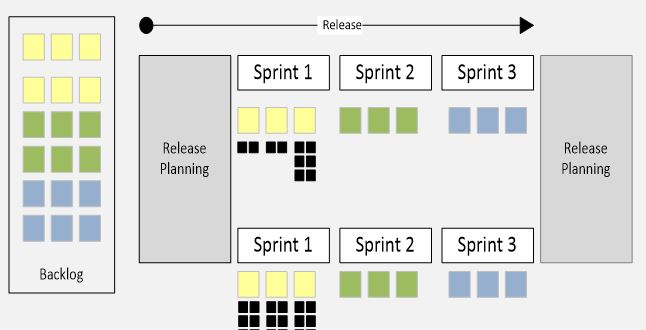
\includegraphics[width=\textwidth]{./ressourcen/release-planning.jpg}
	\caption{Release Planung}
	Source: \url{https://www.scrumdesk.com/wp-content/uploads/Release-planning.jpg}
\end{figure}

\subsection{Entwicklungsworkflow}
\begin{figure}[!ht]
	\centering
	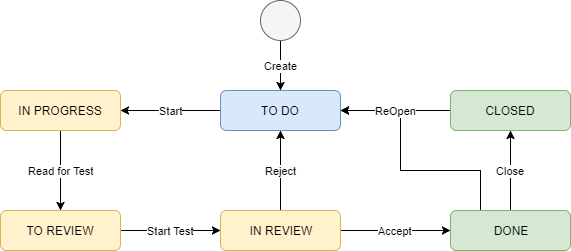
\includegraphics[width=\textwidth]{./ressourcen/entwicklungs-workflow.png}
	\caption{Entwicklungs Workflow}
\end{figure}
Eine Aufgabe/User Story/Epic durchläuft in der Entwicklungsphase immer einen gleichen Workflow. Während diesem Workflow können verschiedene Status erreicht werden:
\begin{description}
	\item[To Do] Aufgabe muss bearbeitet werden
	\item[In Progress] Aufgabe wird derzeitig bearbeitet
	\item[To Review] Aufgabe wurde bearbeitet und kann nun getestet werden
	\item[In Review] Aufgabe wird derzeitig getestet
	\item[Done] Die Aufgabe ist getestet und fertig gestellt
	\item[Closed] Die Aufgabe ist endgültig abgeschlossen (Sprint in welchen die Aufgabe lag ist fertig)
\end{description}
Erstellt man eine Aufgabe wird dieser automatisch der Status "`To Do"' zugewiesen. Aus dem Status "`To Do"' kann nun eine Aufgabe durch starten in den "`In Progress"' Zustand versetzt werden. Ist man nun fertig mit der Implementierung kann man die Aufgabe für das Testen bereit geben in dem man die Aufgabe in "`To Review"' verschiebt. Fängt eine Person an die Aufgabe zu testen verschiebt man diese in "`In Review"', wo man die Aufgabe entweder ablehnen (Status zu "`To Do"' ändern) oder annehmen (Status zu "`Done"' ändern) kann. Sind trotz der Kontrolle noch Fehler in der Aufgabe vorhanden so kann diese von Done/Closed immer wieder in den "`To Do"' Status versetzt werden. Die Transition von "`Done"' zu "`Closed"' erfolgt sobald eine Sprint abgeschlossen ist.
